\chapter{BDT Discriminant}
\label{ch:BDT}

The Toolkit for Multivariate Data Analysis with ROOT (TMVA) package is used to perform BDT training~\cite{Hocker:2007ht}. This ROOT-integrated library enables the usage of the machine learning techniques for the physics data analysis and is commonly used. 

\section{Construction of the BDT}
In this analysis we use the set of nine variables to construct the BDT. These variables are the same in both low and high mass trainings and for both heavy resonances.

Some variables are important only in the specific mass regime, some are ranked highly universally across the whole mass range. For example, in the low mass regime \ETmiss and \HBB~ mass are powerful discriminators against Drell-Yan to leptons plus jets. That is why these
observables are located in the top three variables of the ranking for low mass BDT (Figs. ~\ref{fig:ranking}). In the high mass regime the leverage is in the boost, therefore, $\Delta R = \sqrt{\Delta \phi^2 + \Delta \eta^2}$ variables, as well as $p_{T}$-related variables show high performance (Figs. ~\ref{fig:ranking}). Namely, $p_{T}$ of both Higgs bosons, Z boson, and also
separation $\Delta R $  between two b-jets and also $\Delta R$ between  two leptons. It is worth noting that \HBB~ mass is a powerful discriminator ranked highly for all mass regimes and both channels. Plots of input variables and correlations are shown on the Figs. ~\ref{fig:ele_lowVars}, ~\ref{fig:muon_lowVars}, ~\ref{fig:ele_cors_low}, ~\ref{fig:ele_cors_high}, ~\ref{fig:muon_cors_low}, ~\ref{fig:muon_cors_high}.

\begin{figure}[tbp]
  \begin{center}
   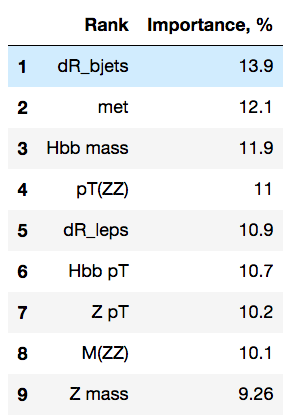
\includegraphics[width=0.35\textwidth]{ee_low.png}
   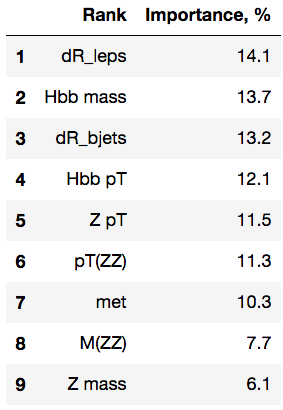
\includegraphics[width=0.35\textwidth]{ee_high.png}\\
   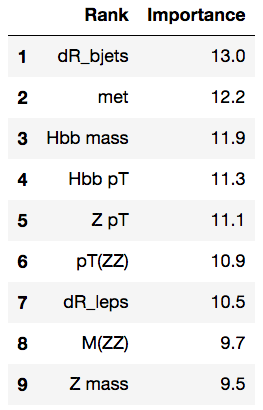
\includegraphics[width=0.35\textwidth]{mm_low.png}
   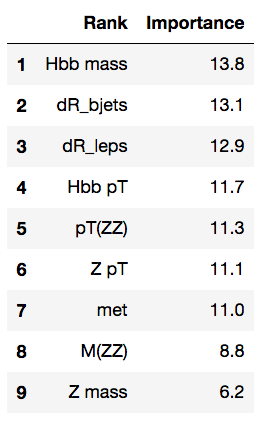
\includegraphics[width=0.35\textwidth]{mm_high.png}
    \caption{ Ranking of variables in the BDT training for electron(muon) channel at the top(bottom). Left: low mass BDT. Right: high mass BDT.}
    \label{fig:ranking}
  \end{center}
\end{figure}


\begin{figure}[tbp]
  \begin{center}
   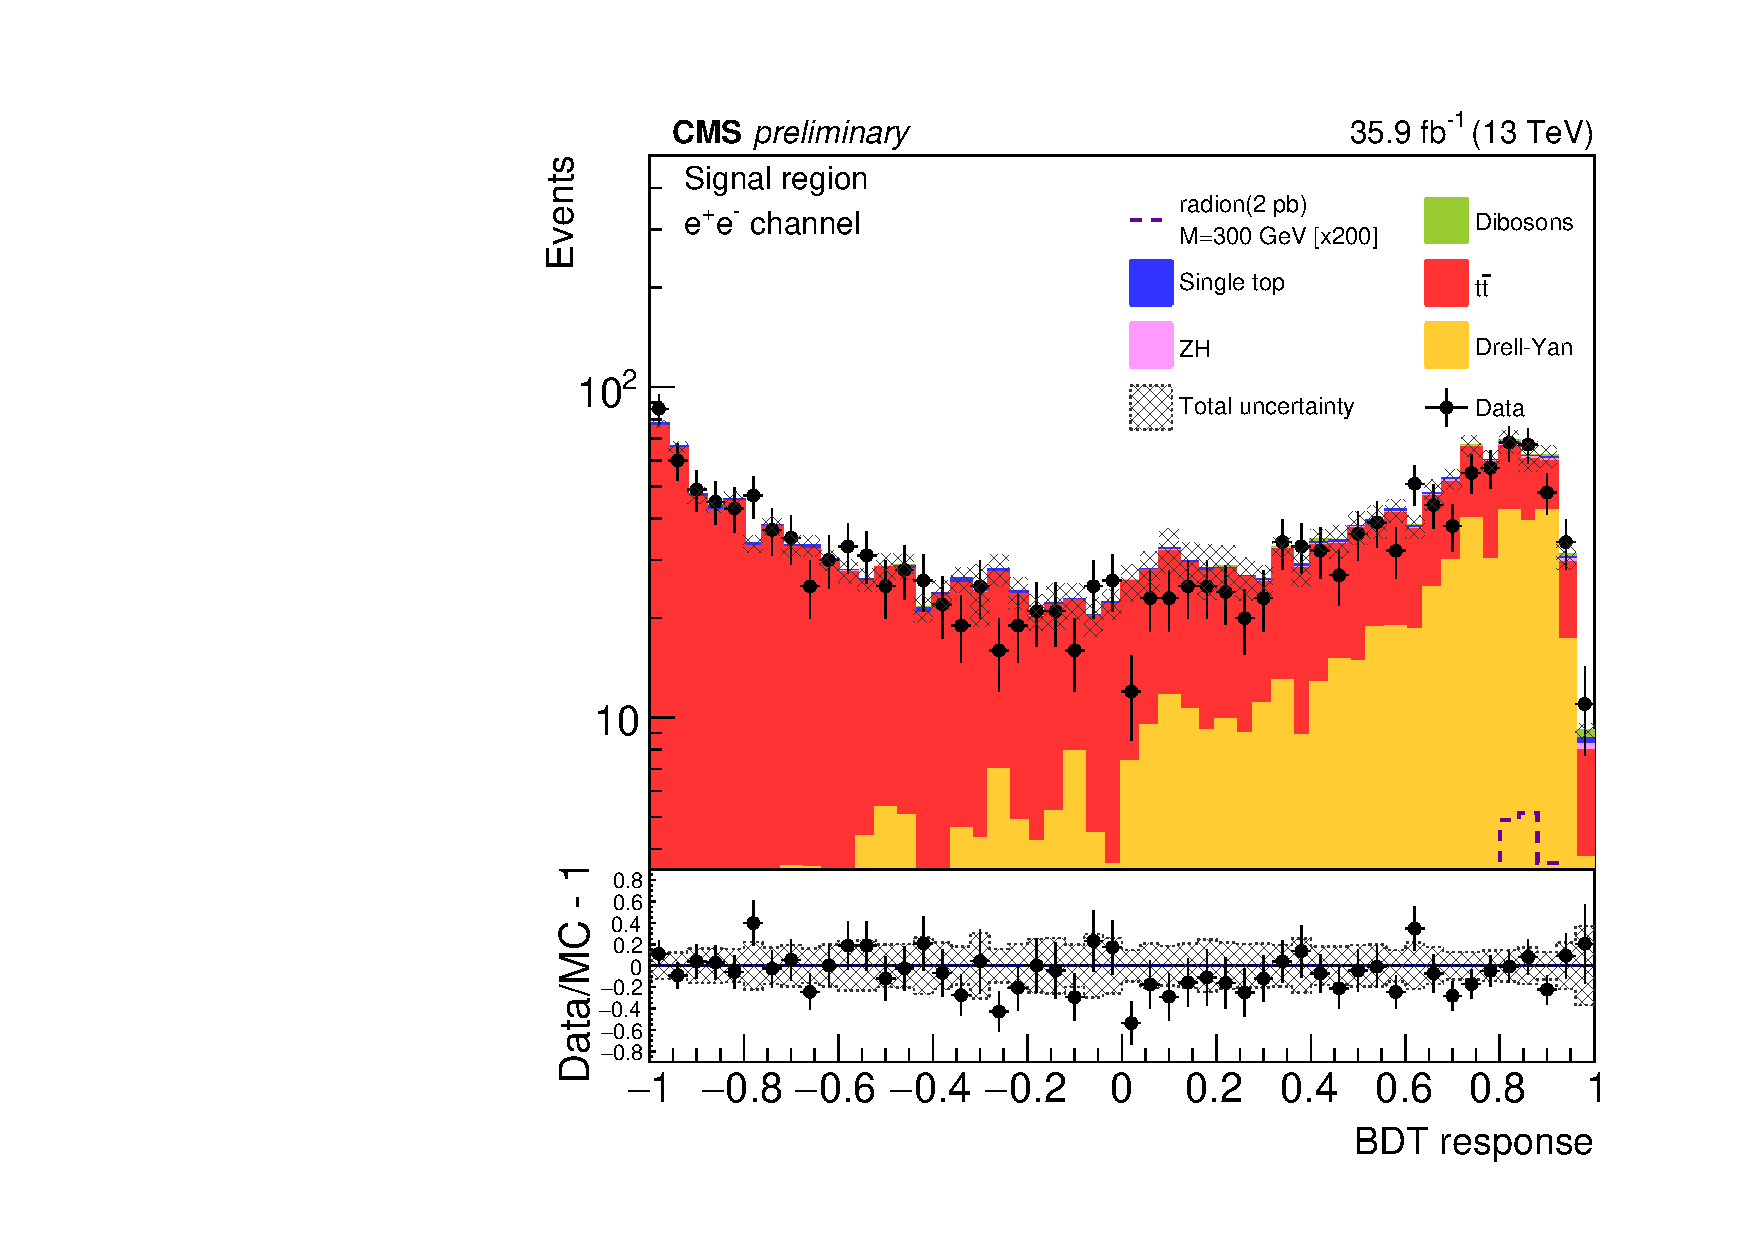
\includegraphics[width=0.6\textwidth]{bdt_response_ee_SR_FullPostfit_plot_nov16_2_radion.pdf}\\
   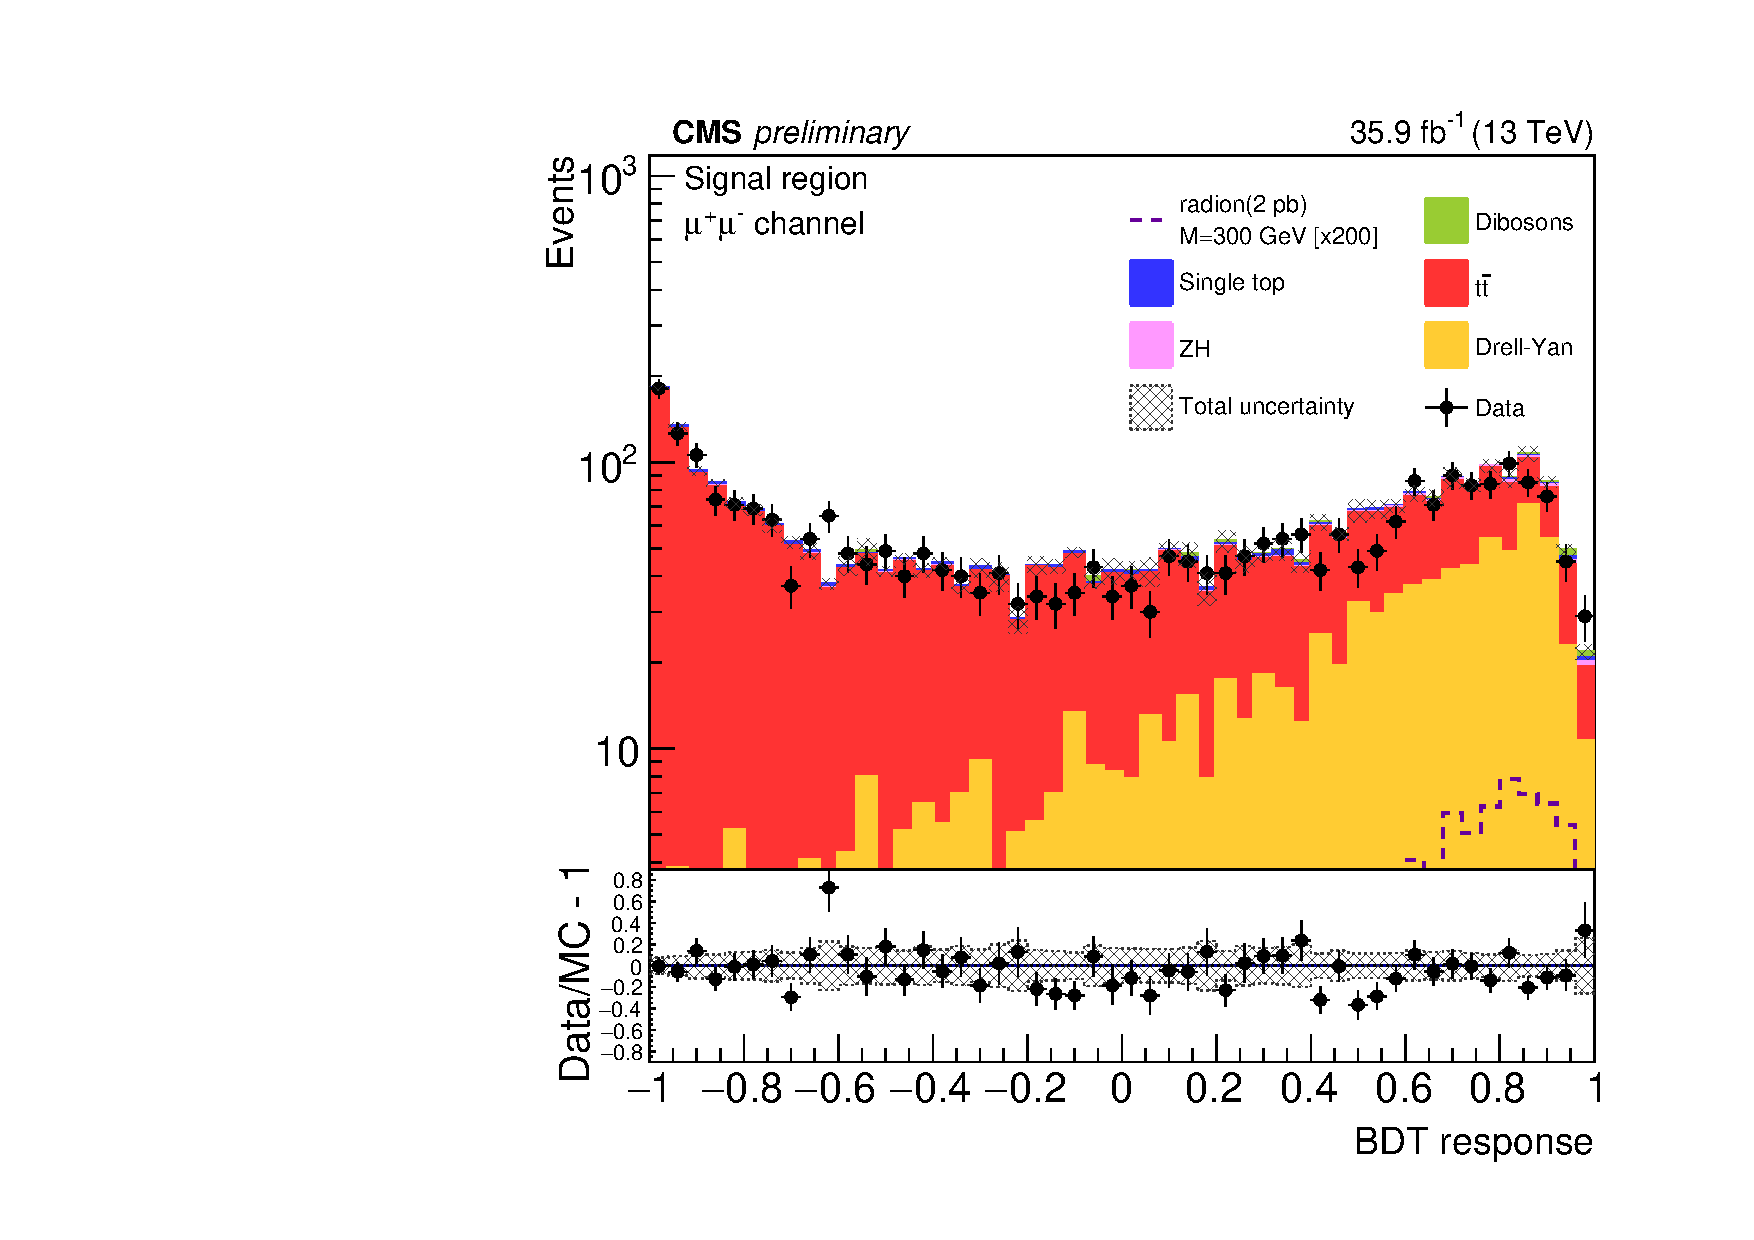
\includegraphics[width=0.6\textwidth]{bdt_response_mm_SR_FullPostfit_plot_nov16_2_radion.pdf}\\
    \caption{ BDT plots for radion case, electron(muon) channel at the top(bottom). Signal region, 300 GeV mass hypothesis. For electrons cut is at 0.4, for muons at 0.7. More details at the table \ref{suboptCut}.}
    \label{fig:BDTs}
  \end{center}
\end{figure}




\begin{figure}[tbp]
  \begin{center}
   \includegraphics[width=0.95\textwidth]{bdtPlots_eles/low_vars1.pdf}
   \includegraphics[width=0.95\textwidth]{bdtPlots_eles/low_vars2.pdf}
    \caption{ Variables used in the low mass training for electron channel. Index '1' refers to \bbbar and index '0' refers to ZZ.}
    \label{fig:ele_lowVars}
  \end{center}
\end{figure}



\begin{figure}[tbp]
  \begin{center}
   \includegraphics[width=0.95\textwidth]{bdtPlots_eles/high_vars1.pdf}
   \includegraphics[width=0.95\textwidth]{bdtPlots_eles/high_vars2.pdf}
    \caption{ Variables used in the high mass training for electron channel.}
    \label{fig:ele_highVars}
  \end{center}
\end{figure}


It is hard to get high performance in the low mass training, since
this is where all the backgrounds are concentrated (Figs. ~\ref{fig:ele_lowVars}, ~\ref{fig:muon_lowVars}). The rate of background in this region is enormous and most variables have similar distributions for signal and backgrounds. However, BDT performance is noticeably better than what can be achieved using a simple linear discriminant method (Figs. ~\ref{fig:ele_BDTs}, ~\ref{fig:ele_ROCs}, ~\ref{fig:muon_BDTs}, ~\ref{fig:muon_ROCs}). 

Earlier versions of the analysis tried more granular approach to the number of BDTs, up to four BDTs to cover the whole range from 250 to 1000 GeV. But it was shown that this added extra complexity brings almost no improvement, while in fact is error prone and computationally twice more expensive. This is why other HH analyses also split the whole mass range only in two subranges and we followed the same suggestion. The BTD plots for radion case in the signal regions for 300 GeV mass hypothesis are shown at Fig. \ref{fig:BDTs}.



\begin{figure}[tbp]
  \begin{center}
   \includegraphics[width=0.75\textwidth]{bdtPlots_eles/low_bdt.pdf}
   \includegraphics[width=0.75\textwidth]{bdtPlots_eles/high_bdt.pdf}
    \caption{ BDT discriminants for electron channel. Top: low mass training. Bottom: high mass training. }
    \label{fig:ele_BDTs}
  \end{center}
\end{figure}

Performance of the high mass training is perfect (Figs. ~\ref{fig:ele_highVars}, ~\ref{fig:muon_highVars}, ). The ROC curves are close to the top right corner of the efficiencies space, which means a high signal efficiency is achieved along side with the low efficiency of the background. This is due to the
fact that most backgrounds peak in the low mass region. Even linear
discriminant is performing well in this situation (Figs. ~\ref{fig:ele_BDTs}, ~\ref{fig:ele_ROCs}, ~\ref{fig:muon_BDTs}, ~\ref{fig:muon_ROCs}).

\begin{figure}[tbp]
  \begin{center}
   \includegraphics[width=0.75\textwidth]{bdtPlots_eles/low_roc.pdf}
   \includegraphics[width=0.75\textwidth]{bdtPlots_eles/high_roc.pdf}
    \caption{ ROC curves for electron channel. Top: low mass training. Bottom: high mass training. }
    \label{fig:ele_ROCs}
  \end{center}
\end{figure}

\begin{figure}[tbp]
  \begin{center}
   \includegraphics[width=0.75\textwidth]{bdtPlots_eles/low_corS.pdf}
   \includegraphics[width=0.75\textwidth]{bdtPlots_eles/low_corB.pdf}
    \caption{ Input variables correlations for electron channel, low mass training. Top: signal sample mix. Bottom: background sample mix. }
    \label{fig:ele_cors_low}
  \end{center}
\end{figure}


\begin{figure}[tbp]
  \begin{center}
   \includegraphics[width=0.75\textwidth]{bdtPlots_eles/high_corS.pdf}
   \includegraphics[width=0.75\textwidth]{bdtPlots_eles/high_corB.pdf}
    \caption{ Input variables correlations for electron channel, high mass training. Top: signal sample mix. Bottom: background sample mix. }
    \label{fig:ele_cors_high}
  \end{center}
\end{figure}


For completeness purpose and research reproducibility, it is worth mentioning in this paragraph the technical details. The following TMVA specific parameters have been used for the BDT training (most parameters are default ones since no significant improvement was observed when varying the parameters one at a time): NTrees = 800, BoostType=Grad, Shrinkage=0.1, UseBaggedBoost=True, GradBaggingFraction=0.5, SeparationType= GiniIndex, nCuts=30, and MaxDepth=3. %Few modifications did not improve much the performance.


Electrons and muons have been optimised separately but BDT trainings show similar performance (Fig. ~\ref{fig:ele_ROCs} and ~\ref{fig:muon_ROCs}). BDT distributions for data and MC comparison are created with the nominal values for the lepton and b jet scale factors. When shape systematics is considered to produce final limits, BDT shapes are
varied using 'Up' or 'Down' versions of the scale factors and all the input variables to the BDT are modified in the similar fashion as well. The BDT plots shown below are further modified applying postfit values of DY and \ttbar normalizations returned from the Maximum Likelihood fit performed with the real data. 



%% \begin{figure}[tbp]
%%   \begin{center}
%%    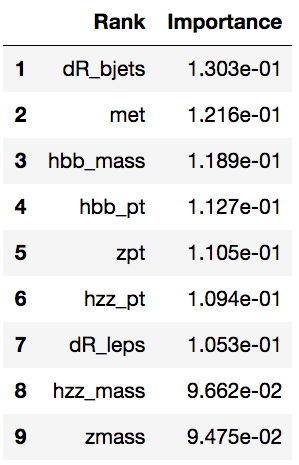
\includegraphics[width=0.35\textwidth]{low_muon.png}
%%    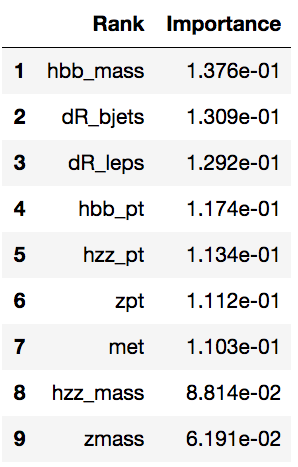
\includegraphics[width=0.35\textwidth]{high_muon.png}
%%     \caption{ Ranking of variables in the BDT training for muon channel. Left: low mass BDT. Right: high mass BDT.}
%%     \label{fig:muon_ranking}
%%   \end{center}
%% \end{figure}



\begin{figure}[tbp]
  \begin{center}
   \includegraphics[width=0.95\textwidth]{bdtPlots_muons/low_vars1.pdf}
   \includegraphics[width=0.95\textwidth]{bdtPlots_muons/low_vars2.pdf}
    \caption{Variables used in the low mass training for muon channel. Index '1' refers to \bbbar and index '0' refers to ZZ.}
    \label{fig:muon_lowVars}
  \end{center}
\end{figure}



\begin{figure}[tbp]
  \begin{center}
   \includegraphics[width=0.95\textwidth]{bdtPlots_muons/high_vars1.pdf}
   \includegraphics[width=0.95\textwidth]{bdtPlots_muons/high_vars2.pdf}
    \caption{ Variables used in the high mass training for muon channel.}
    \label{fig:muon_highVars}
  \end{center}
\end{figure}


\begin{figure}[tbp]
  \begin{center}
   \includegraphics[width=0.75\textwidth]{bdtPlots_muons/low_bdt.pdf}
   \includegraphics[width=0.75\textwidth]{bdtPlots_muons/high_bdt.pdf}
    \caption{ BDT discriminants for muon channel. Top: low mass training. Bottom: high mass training. }
    \label{fig:muon_BDTs}
  \end{center}
\end{figure}

\begin{figure}[tbp]
  \begin{center}
   \includegraphics[width=0.75\textwidth]{bdtPlots_muons/low_roc.pdf}
   \includegraphics[width=0.75\textwidth]{bdtPlots_muons/high_roc.pdf}
    \caption{ ROC curves for muon channel. Top: low mass training. Bottom: high mass training. }
    \label{fig:muon_ROCs}
  \end{center}
\end{figure}

\begin{figure}[tbp]
  \begin{center}
   \includegraphics[width=0.75\textwidth]{bdtPlots_muons/low_corS.pdf}
   \includegraphics[width=0.75\textwidth]{bdtPlots_muons/low_corB.pdf}
    \caption{ Input variables correlations for muon channel, low mass training. Top: signal sample mix. Bottom: background sample mix. }
    \label{fig:muon_cors_low}
  \end{center}
\end{figure}


\begin{figure}[tbp]
  \begin{center}
   \includegraphics[width=0.75\textwidth]{bdtPlots_muons/high_corS.pdf}
   \includegraphics[width=0.75\textwidth]{bdtPlots_muons/high_corB.pdf}
    \caption{ Input variables correlations for muon channel, high mass training. Top: signal sample mix. Bottom: background sample mix. }
    \label{fig:muon_cors_high}
  \end{center}
\end{figure}


